\documentclass[conference]{IEEEtran}
\IEEEoverridecommandlockouts
% The preceding line is only needed to identify funding in the first footnote. If that is unneeded, please comment it out.
\usepackage[hidelinks]{hyperref}
\urlstyle{same}
\usepackage[spanish,es-tabla]{babel}
\usepackage{cite}
\usepackage{amsmath,amssymb,amsfonts}
\usepackage{algorithmic}
\usepackage{graphicx}
\usepackage{textcomp}
\usepackage{xcolor}
\decimalpoint
\renewcommand{\labelitemi}{$\bullet$}
\def\BibTeX{{\rm B\kern-.05em{\sc i\kern-.025em b}\kern-.08em
    T\kern-.1667em\lower.7ex\hbox{E}\kern-.125emX}}
    
    
 %-------------------------------------------------------------------------------
%                            Libreria de codigos                               %
%-------------------------------------------------------------------------------
% Paquetes necesarios
\usepackage{listings}
\usepackage{xcolor}
\usepackage{comment}

% Tipos de letra personalizadas
\def\lstbasicfont{\fontfamily{pcr}\selectfont\scriptsize}
\def\vhdlbasicfont{\fontfamily{cmtt}\selectfont\scriptsize}

% Colores personalizados
\definecolor{codegreen}{rgb}{0,0.6,0}
\definecolor{codepurple}{rgb}{0.58,0,0.82}

\definecolor{codegray}{rgb}{0.5,0.5,0.5}
\definecolor{backcolour}{rgb}{0.95,0.95,0.92}
\definecolor{codeorange}{RGB}{254, 100, 35}

% Deficion de lenguajes perzonalizados

% Definicion de lenguaje MATLAB
\lstdefinelanguage{matlabfloz}{%
  alsoletter={...},%
  morekeywords={%                             % keywords
		break,case,catch,classdef,continue,else,
		elseif,end,for,function,global,if,
		otherwise,parfor,persistent,
		return,spmd,switch,try,while,...},        % Use the matlab "iskeyword" command to get those
  comment=[l]\%,                              % comments
  morecomment=[l]...,                         % comments
  morecomment=[s]{\%\{}{\%\}},                % block comments
  morestring=[m]'                             % strings 
}[keywords,comments,strings]%

% Estilos MATLAB
\lstdefinestyle{MATLAB}{
	frame=single,
	rulecolor=\color{black},
	framexleftmargin=4mm,
	xleftmargin=2mm,
	language=matlabfloz,
  commentstyle=\color{codegreen},
  keywordstyle=\color{blue}, %magenta
  numberstyle=\tiny\color{black},
  stringstyle=\color{codepurple},
  basicstyle=\lstbasicfont\scriptsize,
  breakatwhitespace=false,         
  breaklines=true,                 
  captionpos=b,                    
  keepspaces=true,                 
  numbers=left,                    
  numbersep=5pt,                  
  showspaces=false,                
  showstringspaces=false,
  showtabs=false,                  
  tabsize=2    
}

\lstdefinestyle{PYTHON}{
	frame=single,
	rulecolor=\color{black},
	framexleftmargin=5mm,
	xleftmargin=10mm,
	language=python,
    backgroundcolor=\color{backcolour},   
    commentstyle=\color{codegreen},
    keywordstyle=\color{blue}, %magenta
    numberstyle=\tiny\color{black},
    stringstyle=\color{codeorange},
    basicstyle=\lstbasicfont\footnotesize,
    breakatwhitespace=false,         
    breaklines=true,                 
    captionpos=b,                    
    keepspaces=true,                 
    numbers=left,                    
    numbersep=5pt,                  
    showspaces=false,                
    showstringspaces=false,
    showtabs=false,                  
    tabsize=2,
    otherkeywords = {show,arange}  
}


\lstdefinestyle{CC}{
	frame=single,
	rulecolor=\color{black},
	framexleftmargin=5mm,
	xleftmargin=10mm,
	language=c++,
    backgroundcolor=\color{backcolour},   
    commentstyle=\color{codegreen},
    keywordstyle=\color{blue}, %magenta
    numberstyle=\tiny\color{black},
    stringstyle=\color{codeorange},
    basicstyle=\lstbasicfont\footnotesize,
    breakatwhitespace=false,         
    breaklines=true,                 
    captionpos=b,                    
    keepspaces=true,                 
    numbers=left,                    
    numbersep=5pt,                  
    showspaces=false,                
    showstringspaces=false,
    showtabs=false,                  
    tabsize=2,
    otherkeywords = {show,arange}  
}


\lstdefinestyle{BASH}{
	frame=single,
	rulecolor=\color{black},
	framexleftmargin=4mm,
	xleftmargin=2mm,
	language=bash,
    %backgroundcolor=\color{backcolour},   
    commentstyle=\color{codegreen},
    keywordstyle=\color{blue}, %magenta
    numberstyle=\tiny\color{black},
    stringstyle=\color{codeorange},
    basicstyle=\lstbasicfont\footnotesize,
    breakatwhitespace=false,         
    breaklines=true,                 
    captionpos=b,                    
    keepspaces=true,                 
    numbers=left,                    
    numbersep=5pt,                  
    showspaces=false,                
    showstringspaces=false,
    showtabs=false,                  
    tabsize=2,
    %otherkeywords = {show,arange}  
}

\renewcommand{\lstlistingname}{Código}% Listing -> Algorithm
\renewcommand{\lstlistlistingname}{Lista de códigos}% 
\begin{document}

\title{Tarea 6: Linearización de la transconductancia de un OTA a través del algoritmo NSGA-II.
}

\author{\IEEEauthorblockN{Ciro Fabian Bermudez Marquez}
INAOE\\
Mexico, Puebla \\
\url{cirofabian.bermudez@gmail.com}
}

\maketitle

\begin{abstract}
En este trabajo se optimiza un circuito OTA utilizando la metodología vista en clase y el algoritmo de NSGA-II.
\end{abstract}



\section{Descripción del problema}

Utilizar ngspice y los programas proporcionados en clase para resolver el problema de optimización de linearizar la transconductancia de un OTA utilizando NSGA-II.

El circuito que se optimizará es el siguiente:

\begin{figure}[hbtp]
\centering
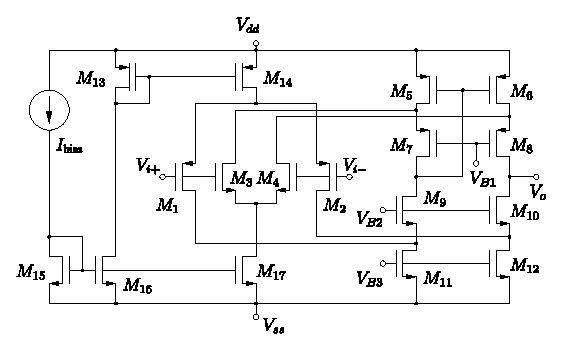
\includegraphics[width=0.45\textwidth]{circuito.eps}
\caption{Amplificador cascode.}
\end{figure}

Utilizar la semilla 0.1234 y analizar para 100, 150 y 200 generaciones con $\eta_{c}$: 20 y  $\eta_{m}$: 20.

\section{Resultados}

El archivo \textbf{input.txt} se configuró de la siguiente manera:

\begin{itemize}
\item Tamaño de población: 100
\item Número de generaciones: 100, 150, 200
\item Número de objetivos: 2
\item Número de restricciones: 16
\item Número de variables reales: 5
\item Rango de la variable $x_{1},x_{2}, \cdots ,x_{5}$: $[ 1,100]$
\item Probabilidad de cruza: 0.9
\item Probabilidad de mutación: 0.5
\item Índice de distribución para el cruce SBX variable real $\eta_{c}$:   20 
\item Índice de distribución para la mutación polinomial variable real $\eta_{m}$: 20
\item Número de variables binarias: 0
\end{itemize}


En las Figuras \ref{fig:tanaka1}, \ref{fig:tanaka2}, \ref{fig:tanaka3} se muestran los frentes de Pareto obtenidos con las diferentes generaciones.

\begin{figure}[hbtp]
\centering
\includegraphics[width=7cm]{100.pdf}
\caption{Frente de Pareto ancho de banda vs ganancia 100 generaciones.}
\label{fig:tanaka1}
\end{figure}

\begin{figure}[hbtp]
\centering
\includegraphics[width=7cm]{150.pdf}
\caption{Frente de Pareto ancho de banda vs ganancia 150 generaciones.}
\label{fig:tanaka2}
\end{figure}

\begin{figure}[hbtp]
\centering
\includegraphics[width=7cm]{200.pdf}
\caption{Frente de Pareto ancho de banda vs ganancia 200 generaciones}
\label{fig:tanaka3}
\end{figure}



\section{Conclusiones}

Dada la complejidad del problema aun estando el algoritmo codificado en C el tiempo de ejecución estuvo entre 8 a 10 minutos, de estas observaciones se puede rescatar que es importante ser muy meticuloso y metódico al momento de estar trabajando, de lo contrario se perderá valioso tiempo. Variando el número de generaciones el frente de Pareto no mostró cambios notorios. Finalmente podemos decir que el algoritmo NSGA-II encontró de manera correcta el frente de Pareto y que resulto una buena herramienta para este tipo de optimizaciones.

\begin{thebibliography}{00}
\bibitem{b1}  Dr. Luis Gerardo de la Fraga. ``Apuntes de clase'' .
\bibitem{b2} Kalyanmoy Deb.``Multi-objetive Optimization using Evolutionary Algoritms'', John Wiley, 1ra Ed.
\end{thebibliography}


\end{document}
